

\section{Electromyography} \label{sec:BG:EMG}

This project will utilize the method of electromyography to record the muscle activation of the lower arm muscles in relation to the gestures presented in \secref{sec:BG:anatomy} on anatomy. To develop theoretical background knowledge, a short introduction of the essentials of the signal will be presented. 

Electromyography is the recording of muscle activity based on the amount of electrical stimulation. The amount of activity is found by measuring the electric potential, an action potential causing a muscle contraction. The process of planning and executing a voluntary movement starts at the motor cortex in the brain, where a nerve impulse is send and travel through the spinal cord to the lower motor neuron. As seen in \figref{fig:motor} the path from alpha motor neuron through the axon to the motor endplates is what makes up a motor unit. The alpha motor neuron originates from the spinal cord along the axon to the muscle it controls. The axon branches out to multiple muscle fibers through motor endplates innervating the muscle fibers.
%Muscle movement demanding high precision have a higher innervation of motor units than muscles used for more powerful movements. 

\begin{figure}[H]                                         
	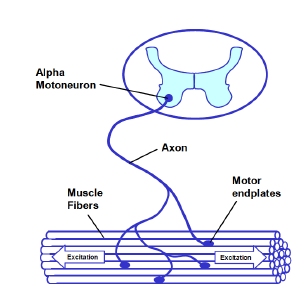
\includegraphics[width=.4\textwidth]{figures/motor_unit}  
	\caption{The figure illustrates the neural pathway from the alpha motor neuron to the innervated muscle fibers, making up a motor unit.\cite{Konrad2005}}
	\label{fig:motor} 
\end{figure}  

The essentials of understanding the application EMG is the excitation of muscle cells. The excitability of the muscle fibers play a crucial role in a muscle contraction. The mechanisms of a contraction can be understood through a series of events. First the muscle cell membrane is at a resting potential between -80 to -90 mV, due to an equilibrium of NA$^+$ and K$^+$ through the intracellular and extracellular side of the membrane, maintained by an ion pump. The before mentioned alpha motor neuron reaches the motor endplates where a transmitter substance is released. The substance alters the membrane characteristics and allows a greater flow of Na$^+$ into the cell. This causes a membrane depolarization, changing the membrane potential. If a threshold between -55 mV to -50 mV is reached excitation in the form of an action potential is formed, travelling in both directions of the muscle fiber, as seen on \figref{fig:motor}. The membrane potential is quickly restored with a great outflow of Na$^+$, resulting in a repolarization. The action potential from each of the activated muscle fibers summates spatially and temporally forming a motor unit action potential (MUAP). The spread of the MUAP over the muscle membrane is recorded with EMG. The number of recruited motor units is a way of controlling the force of a muscle contraction depending on the force needed. Like the recruitment of motor units, the frequency of activation can be modulated for generating a specific amount of force. A higher activation frequency leads to a higher generated force, but this also makes the muscle more prone to fatigue. The number of motor units innervating muscle fibers depend on the muscle characteristics and the purpose is serves. A low innervation ratio between motor units and muscle fibers make up the opportunity of fine motor tasks, while a low ratio is ideal for tasks demanding strength. Furthermore the motor units are recruited in an asynchronous pattern. This further facilitates the possibility of smooth muscle movements. \cite{Martini2012, Cram2012} \fxnote{Jakob would like us to elaborate more on the relation between muscle contractions and the way the EMG signal looks like}

Recording EMG can be done either through the most often used surface EMG (sEMG) or by intra vascular EMG (iEMG). In iEMG a needle is inserted into the muscle measuring the MUAP directly on site. The more often used sEMG uses electrodes measuring the MUAP on the skin surface and will be used to acquire EMG signals in this project. \cite{Cram2012} 
